\documentclass[german,ignorenonframetext]{beamer}

\usepackage[ngerman]{babel} % f�r deutsche Spracheinstellungen
\usepackage{graphics} % um Bilder einbinden zu k�nnen
\usepackage[dvips]{epsfig} % um Bilder zu skalieren
\usepackage[applemac]{inputenc} % inputencoding (MacOS) f�r Umlaute und Akzente
\usepackage{multimedia}

%%%%%%%%%%%%%%%%%%%%%%%%%%%%%%%%%%%%%%%%%%%

%%%%%%% Die folgenden Befehle definieren das Grundlayout, blenden auf der
%%%%%%% Titelseite die HAW-Infos ein und setzen das 
%%%%%%% HAW-Logo in die Ecke
\mode<presentation>{\usetheme{Berkeley}}
\logo{\pgfimage[height=1.5cm]{HAW_wuerfel+}}
\institute[MT -- HAW Hamburg]{HAW Hamburg\\ Fakult�t DMI, Dept.\ Medientechnik}

%%%%%%% der folgende Befehl l�sst die mit "\pause" verdeckten Teile der Folien 
%%%%%%% transparent erscheinen.  
\setbeamercovered{transparent}  

%%%%%%% die folgende Sequenz blendet mit jeder neuen Section einmal das 
%%%%%%% Inhaltsverzeichnis mit dem Titel "�bersicht" ein und markiert den
%%%%%%% jeweils aktuellen Gliederungspunkt
\AtBeginSection[]{
\begin{frame}<beamer>
\frametitle{�bersicht} 
\tableofcontents[currentsection,currentsubsection]
\end{frame}
}

%%%%%%%%%%%%%%%%%%%%%%%%%%%%%%%%%%%%%%%%%%%

%%%%%%% jeder dieser Titelseiten-Befehle kennt eine in eckige Klammern gesetzte 
%%%%%%% Kurzform, die im Rand benutzt wird
\title[�berschrift]{Die Haupt�berschrift}
\subtitle{Und eine Unter--�berschrift}
\author[Name]{Vorname Nachname}
\date{\today}

%%%%%%%%%%%%%%%%%%%%%%%%%%%%%%%%%%%%%%%%%%%

\begin{document}

%%%%%% dieser Befehl erzeugt das Deckblatt. 
%%%%%% Mit der Option plain wird das Layout f�r das Deckblatt abgeschaltet
%\frame[plain]{\titlepage}
\frame{\titlepage}

\begin{frame}
  \frametitle{�bersicht}
  \tableofcontents
\end{frame}

%%%%%%%%%%%%%%%%%%%%%%%%%%%%%%%%%%%%%%%%%%%
\section{Emotiv Epoc} % die sections sind hier nur zum Strukturieren des Vortrags!!
%% der Name der section taucht nur im Inhaltsverzeichnis und im linken Rand auf.
%%%%%%%%%%%%%%%%%%%%%%%%%%%%%%%%%%%%%%%%%%%

\begin{frame}
  \frametitle{Emotiv-API}
  
  \pgfimage[width=\textwidth]{EmoEngine}
  

\end{frame}

\begin{frame}
  \frametitle{Emotiv-API}
  
  Die Emotiv-API (drei C-Header und entsprechende Binaries) bietet Zugriff auf Daten auf vier veschiedenen Ebenen:
  
\begin{enumerate}
\item rohe Messwerte der 14 Elektroden und des Gyroskops
\item Mimik-Ereignisse (''Expressiv Suite'')
\item ''Emotions-Werte'' (''Affectiv Suite'')
\item trainierte, wiedererkannte ''Gedanken''-Muster (''Cognitiv Suite'')
\end{enumerate} 

Wie die Daten der Ebenen 2-4 berechnet werden, bleibt leider ein Geheimnis der Hersteller-Firma.

\end{frame}



%%%%%%%%%%%%%%%%%%%%%%%%%%%%%%%%%%%%%%%%%%%
\section{Datenanalyse} 
%%%%%%%%%%%%%%%%%%%%%%%%%%%%%%%%%%%%%%%%%%%

\begin{frame}
\frametitle{Video ''linkes Bein''}
\movie[externalviewer]{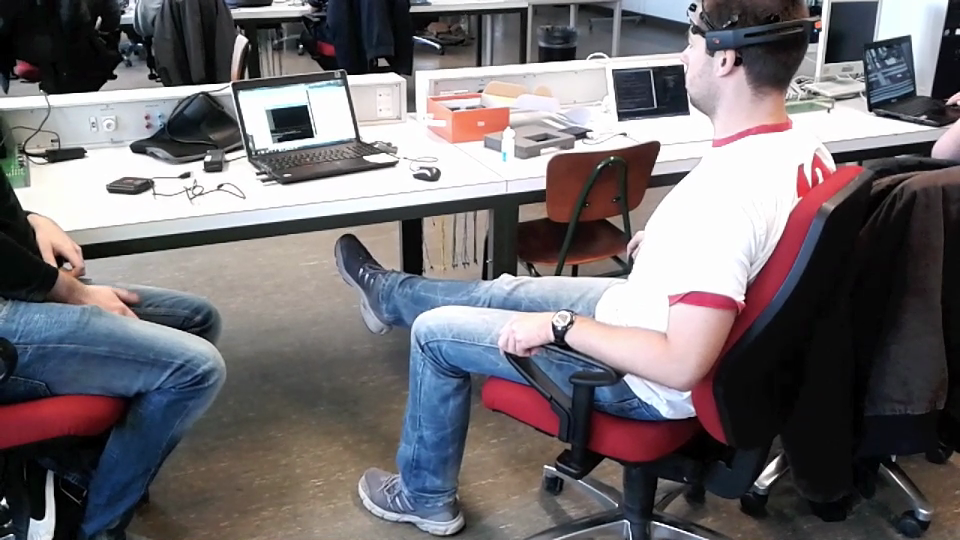
\includegraphics[width=\textwidth]{Snapshot_linkes_Bein.png}} {Video_linkes_Bein_edit.mov} %% Snapshot �ndern!!!!
\end{frame}

\begin{frame}
\frametitle{Auswertung - erste Versuche}
  
\pgfimage[width=\textwidth]{linplot_linkes_bein.png}
  
\end{frame}

\begin{frame}
\frametitle{Auswertung - mit bwview}
 
\begin{center}  
\pgfimage[width=\textwidth]{Video_linkes_Bein_bfview.png}
\end{center}  
\end{frame}



\end{document} %%%%% END DOCUMENT %%%%%%


%%%%%%%%%%%%%%%%%%%%%%%%%%%%%%%%%%%%%%%%%%%
%%  besondere Gestaltungselemente f�r Vortragsfolien
%%%%%%%%%%%%%%%%%%%%%%%%%%%%%%%%%%%%%%%%%%%

% Folie
\begin{frame}
\frametitle{Folientitel}
        Text, Bilder, Bl�cke
\end{frame}

% neutraler Kasten
\begin{block}{Blocktitel}
        Blocktext
\end{block}

% gr�ner Kasten
\begin{exampleblock}{Beispielblocktitel}
        Beispielblocktext
\end{exampleblock}

% roter Kasten
\begin{alertblock}{Warnungsblocktitel}
        Warnungsblocktext
\end{alertblock}

% mehrspaltige Folie mit variablen Spaltenbreiten
\begin{columns}
\column{.55\textwidth}
        Text oder Bild
\column{.45\textwidth}
        Text oder Bild
\end{columns}

% sukzessiver Folienaufbau 
\pause

% mehr Befehle f�r sukzessiven Folienaufbau, 
% der geklammerte Teil erscheint jeweils ab der dritten Teil-Folie
\uncover<3->{}
\only<3->{}
\invisible<1-2>{}

% rote Markierung des geklammerten Teils bei der vierten Teil-Folie
\alert<4>{}

%%%%%%%%%%%%%%%%%%%%%%%%%%%%%%%%%%%%%%%%%%%